
% \documentclass[10pt,letterpaper,twocolumn]{article}
\documentclass[conference, letterpaper, 10pt, twocolumn]{cls/IEEEtran}
% {technote, conference, journal, peerreview}

% Margins
\usepackage[margin=.5in]{geometry} % corrects the margins
%\newcommand{\CLASSINPUTinnersidemargin}{0.70in} % inner side margin
%\newcommand{\CLASSINPUToutersidemargin}{0.70in} % outer side margin
%\newcommand{\CLASSINPUTtoptextmargin}{0.75in} % top text margin
%\newcommand{\CLASSINPUTbottomtextmargin}{0.75in} % bottom text margin

% Space Adjustments
%\addtolength{\textfloatsep}{-2mm} % reduce space between figs & text
%\addtolength{\intextsep}{-2mm}	   % reduce space between intext fig & text
%\addtolength{\floatsep}{-5mm}		 % reduce the space between figures
% These are specific to caption package:
%\setlength{\belowcaptionskip}{-3.5pt}
%\setlength{\abovecaptionskip}{3pt}


% Packages
\usepackage[normalem]{ulem}	                        % underlining!
\usepackage[table,usenames,dvipsnames]{xcolor}      % color
\usepackage{enumitem}                               % [inline]
\usepackage{extarrows}                              % http://ctan.org/pkg
\usepackage[noadjust]{cite}                         % Citation
%\usepackage[comma]{natbib}
%\usepackage[numbers]{natbib}

% Math
\usepackage{amsmath,amssymb,amsfonts,amsthm,dsfont} % math
\usepackage{algorithm,algorithmicx,listings}        % algorithms
\usepackage[noend]{algpseudocode}			        % necessary for algorithmicx
%\usepackage{mathtools,thmtools}
\usepackage{bm}

% Figures
\usepackage{graphicx,tabularx,subcaption}
\usepackage[export]{adjustbox}% http://ctan.org/pkg/adjustbox
%\usepackage{wrapfig}
%\usepackage{multirow,multicol,array,rotating,diagbox}
%\usepackage{makecell,booktabs}
%\usepackage{subfigure}
%\usepackage{subfig}

\usepackage[font={small}]{caption}
\captionsetup[algorithm]{font=small}
%\usepackage[font={small,sf},labelfont=bf,format=hang,format=plain,margin=0pt,width=0.8\textwidth]{caption}
%\usepackage[font={small}]{subcaption} % list=true


% Appendix stuff
\let\appendices\relax
\usepackage[titletoc,title]{appendix}

% Always import last
\usepackage[breaklinks=true, colorlinks, bookmarks=true, citecolor=Black, urlcolor=Violet,linkcolor=Black]{hyperref}


% Commands
\def\argmin{\mathop{\arg\min}\limits}
\def\argmax{\mathop{\arg\max}\limits}
\newcommand{\longeq}[2]{\xlongequal[\!#2\!]{\!#1\!}}
% #1 = top; #2 = bottom; #3 = inequality (<,>,\leq,\geq)
\newcommand{\longineq}[3]{\overset{#1}{\underset{#2}{#3}}}
\newcommand{\indicator}{\mathds{1}}
\newcommand{\ceil}[1]{\lceil#1\rceil}
\newcommand{\floor}[1]{\lfloor#1\rfloor}
\DeclareMathOperator{\tr}{\mathbf{tr}}
\newcommand{\TODO}[1]{{\color{red}#1}}
\newcommand{\scaleMathLine}[2][1]{\resizebox{#1\linewidth}{!}{$\displaystyle{#2}$}}
\newcommand{\prl}[1]{\left(#1\right)}
\newcommand{\brl}[1]{\left[#1\right]}
\newcommand{\crl}[1]{\left\{#1\right\}}

% Environments:
\newtheorem{theorem}{Theorem}
\newtheorem{proposition}{Proposition}
\newtheorem{corollary}{Corollary}
\newtheorem{lemma}{Lemma}
\theoremstyle{definition}
\newtheorem{definition}{Definition}
\newtheorem{assumption}{Assumption}
\newtheorem*{assumption*}{Assumption}
\newtheorem*{problem*}{Problem}
\newtheorem{problem}{Problem}
\theoremstyle{remark}
\newtheorem{remark}{Remark}
\newtheorem*{solution*}{Solution}


% Meta data
\def\thetitle{Summary: Deterministic Variational Inference for Robust Bayesian Neural Networks}
\def\theauthor{Ibrahim Akbar}
% \def\thekeywords{keywords}

\hypersetup{
  pdfauthor={\theauthor},%
  pdftitle={\thetitle},%
  pdfsubject={\thetitle},%
  % pdfkeywords={\thekeywords}
}

\title{\LARGE \bf \thetitle% <-this % stops a space
% \thanks{We gratefully acknowledge support from ARL RCTA W911NF-10-2-0016.}
}

\author{%
summarized by Ibrahim Akbar
\\
Department of Electrical and Computer Engineering\\
University of California, San Diego\\
%
}
\date{}



%==================================================================%
\begin{document}
\maketitle


\begin{abstract}
This paper considers the problem of variational inference in bayesian neural networks. Specifically, they are concerned with improving the efficiency and robustness of learning priors over the weight space. To do this they introduce a deterministic approximation of the reconstruction term in the ELBO and a general robust method for prior selection from hierarchical priors for the KL Divergence.
\end{abstract}


\section{Introduction}
\label{sec:introduction}

Full bayesian inference for most neural network is intractable due to the model's nonlinearity causing the true posterior distribution to be highly complex. This has led to the use of variational methods which attempt to approximate the posterior. With regard to bayesian variational inference; this paper addresses the general issue of prior selection to reduce the sensitivity BNNs have toward such initializations and the high variance that arises in the gradients when employing Monte Carlo approximation techniques.

The authors list their contributions as:
\begin{itemize}
	\item Development of a deterministic procedure for propagating uncertain activations through neural networks with uncertain weights and ReLU or Heaviside activation functions.
	\item Development of an EB method for principled tuning of weight priors during BNN training.
	\item Experimental results showing the accuracy and efficiency of our method and applicability to heteroscedastic and homoscedastic regression on real datasets.
\end{itemize}    
 

\section{Problem Formulation}
\label{sec:problem_formulation}

Given a model $\mathcal{M}$ parameterized by $\bm{\omega}$ and a dataset $\mathcal{D} = \{(\mathbf{x}_i,\mathbf{y}_i)\}_{i=1}^{\mathbb{N}}$, the inference goal is to determine the posterior distribution $p(\bm{\omega} \mid \mathbf{X}, \mathbf{Y})$ through Bayes' rule. Since this posterior is generally intractable we consider the parameterized variational distribution $q(\bm{\omega};\bm{\theta})$ that is optimal for $\bm{\theta}^*$ in terms of KL Divergence.

$$
\bm{\theta}^* = \argmin_{\bm{\theta}\in\Theta} KL\left[q(\bm{\omega};\bm{\theta})||p(\bm{\omega} \mid \mathbf{X}, \mathbf{Y})\right]
$$

Given a prior, $p(\bm{\omega})$, we can can reformulate this as the evidence lower bound (ELBO):

\begin{equation}
\bm{\theta}^* = \argmax_{\bm{\theta}\in\Theta}\left\{\mathbb{E}_{\bm{\omega}\sim q}\big[\log p(\mathbf{Y} \mid \mathbf{X}, \bm{\omega})\big] - KL\big[q(\bm{\omega};\bm{\theta} || p(\bm{\omega})\big]\right\}
\end{equation}

The goal of this paper is to derive an explicit deterministic approximation of the first term, known as reconstruction term, and choose priors $p(\bm{\omega})$ empirically to increase robustness to the choice of variance parameters.


\section{Deterministic Variational Approach}
There are two main parts for computing the reconstruction term: propagation of distributions through activations to compute $\tilde{q}(\mathbf{a}^L)$, and evaluation of unparameterized log-likelihood $\mathcal{L}$. In Fig~\ref{fig:feed_arch} we can see the general architecture used to accomplish these tasks.

\begin{figure}[H]
\centering
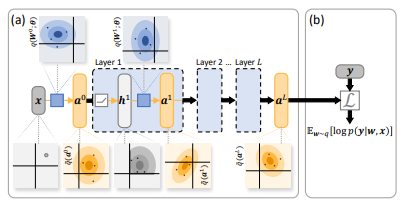
\includegraphics[scale=.5]{fig/dvi-architect-p1.png}
\caption{Feed-forward architecture for reconstruction term computation.}
\label{fig:feed_arch}
\end{figure}

\noindent\textbf{Moment Propagation.} \\
We can consider the model, $\mathcal{M}$, as a set of layers each containing an non-linear and affine transformation,
$$
\mathcal{M} := \{(\bm{h}^l,\bm{a}^l): \bm{h}^l = f(\bm{a}^{l-1}), \bm{a}^l = \bm{h}^l\bm{W}^l + \bm{b}^l\}_{l=1}^{\mathbb{N}}
$$

where $\{\bm{W},\bm{b}\}\subset\bm{\omega}$ are random variables representing the weights and are assumed independent per layer. $\bm{a}^l$ is argued to be Gaussian under the Central Limit Theorem given a sufficiently large latent space and finite $1^{st}$ and $2^{nd}$ moment since it is formulated as the linear combination of the elements of $\bm{h}^l$. Given that $\bm{a}^l$ is Gaussian we can appoximate the $1^{st}$ and $2^{nd}$ moment,

\begin{equation}
\langle a_i\rangle = \langle h_j\rangle\langle W_{ji}\rangle + \langle b_i\rangle
\end{equation}
$$
\text{Cov}(a_i,a_k) = 
$$
\begin{equation}
\langle h_jh_l\rangle\text{Cov}(W_{ji},W_{lk})+ \langle W_{ji}\rangle\text{Cov}(h_j,h_l)\langle W_{lk}\rangle + \text{Cov}(b_i,b_k)
\end{equation}

where $\langle a_i\rangle := \mathbb{E}_{q}[a_i]$ and $h_jW_{ji} = \sum_{j=1}^nh_jW_{ji}$ is called Einstein notation. To reduce approximation, gaussian distributions are considered for the mean and covariance of the weights so that all that is left determine are the moments $\langle h_j\rangle$ and $\langle h_jh_l\rangle$

\begin{equation}
\langle h_j\rangle \propto \int f(\alpha_j)\exp\bigg[-\frac{(\alpha_j-\langle a_j^{l-1}\rangle)^2}{2\Sigma_{jj}^{l-1}}\bigg]d\alpha_j
\end{equation}

\begin{equation}
\langle h_jh_l\rangle \propto \int f(\alpha_j)f(\alpha_l)\exp\bigg[-\frac{1}{2}\zeta^T\Lambda^{-1}\zeta\bigg]d\alpha_jd\alpha_l
\end{equation}

$$
\zeta = \begin{pmatrix} \alpha_j - \langle a_j^{l-1}\rangle\\ \alpha_l - \langle a_l^{l-1}\rangle\\\end{pmatrix}
$$

$$
\Lambda = \begin{pmatrix} \Sigma_{jj}^{l-1} & \Sigma_{jl}^{l-1}\\ \Sigma_{lj}^{l-1} & \Sigma_{ll}^{l-1}\\\end{pmatrix}
$$

 Closed form solutions exist for (4) when considering Heaviside or ReLU non-linearity for $f$. For (5), we can approximate the moment through,

\begin{equation}
\langle h_jh_l\rangle = S_{jl}^{l-1}\bigg\{A(\mu_j^{l-1},\mu_{l}^{l-1},\rho_{jl}^{l-1})+\exp[-Q(\mu_j^{l-1},\mu_l^{l-1},\rho_{jl}^{l-1})]\bigg\}
\end{equation}

where the key idea is that the asymptotes $A$ of the non-linearities as well as the residuals $Q$ in the form of a polynomial provide a good first order approximation of the moment. Fig~\ref{fig:approx} provides a visual representation of this process. Due to CLT these approximations provide sufficient information for us to explicitly determine $\tilde{q}(\bm{a}^L)$ through sequential distribution propagation.

\begin{figure}[H]
\centering
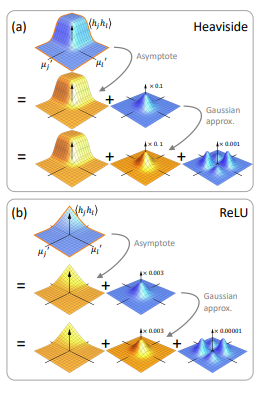
\includegraphics[scale=.5]{fig/activations.png}
\caption{Model activation function approximation.}
\label{fig:approx}
\end{figure}

\noindent\textbf{Log-Likelihood Evaluation.} \\
We can evaluate the expected log-likelihood $\mathbb{E}_{\bm{\omega}\sim q}\big[\log p(y \mid \bm{x},\bm{\omega})\big]$ through directly evaluating $\mathbb{E}_{\bm{a}^L\sim q(\bm{a}^L)}\big[\log p(y \mid \bm{a}^L)\big]$ since $q(y \mid \bm{a}^L)$ is a parameter free transformation.

\section{Empirical Bayes for Variational BNNs}

Considering a $d$-dimensional Gaussian prior, $p(\bm{\omega}) = \mathcal{N}(\mu_p,\Sigma_p)$, and variational distribution, $q = \mathcal{N}(\mu_q,\Sigma_q)$, the KL divergence has the form,

\begin{equation}
\frac{1}{2}\bigg[\log\frac{\det(\Sigma_p)}{\det(\Sigma_q)} - d + \text{tr}(\Sigma_p^{-1}\Sigma_q) + (\mu_p - \mu_q)^T\Sigma_p^{-1}(\mu_p - \mu_q)\bigg]
\end{equation}

Rather than using this directly the authors propose conditioning the prior on a hyper-parameter $\bm{s}$ such that $\bm{\omega}\sim p(\bm{\omega}\mid\bm{s}); \bm{s} \sim p(\bm{s})$, where $\bm{s}$ is distributed according to a inverse gamma distribution and acts as a conjugate prior for the diagonal gaussian variance. Further through partioning the weights $\bm{\omega}$ into sets $\{\lambda\}$ such that an element $s_\lambda$ of $\bm{s}$ can be assigned to each set,
$$
s_\lambda \sim \text{Inv-Gamma}(\alpha,\beta), \quad w_i^\lambda \sim \mathcal{N}(0,s_\lambda) 
$$
we can consider solving the MAP optimization problem for the KL divergence,

$$
s^*_\lambda = \argmin_{s_\lambda} KL\bigg[q(\bm{\omega};\bm{\theta})||p(\bm{\omega}^\lambda\mid s_\lambda) - \log p(s_\lambda)\bigg]
$$

This leads to the closed-form solution,
$$
s^*_\lambda = \frac{\text{tr}(\Sigma_q^\lambda+\mu_q^\lambda(\mu_q^\lambda)^T)+2\beta}{\Omega_\lambda + 2\alpha + 2}
$$

where $\Omega_\lambda := |\lambda|$. We can then use $s^*_\lambda$ to determine the diagonal entries of $\Sigma_p$ and solve (1).

\begin{figure}[H]
\centering
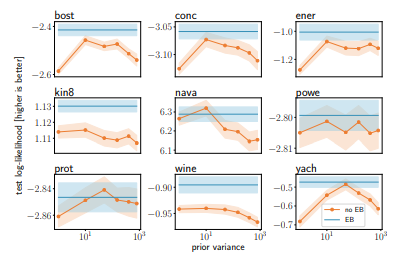
\includegraphics[scale=.5]{fig/empirical-bayes.png}
\caption{Test Log-likelihood with tuned prior (orange) and EB (blue).}
\label{fig:emp_bayes}
\end{figure}

\section{Experiments}

The proposed method, DVI, is evaluated with small networks on UCI datasets in comparison with a large variety of other methods in the Appendix showing that it is capable of performing at the state of art in terms of log-likelihood. Furthermore, the algorithm is also tested extensively on it's own with a variety of configurations in the BNNs to see how the main assumptions hold of CLT, indepdendence, and trunctated polynomial hold. A further study that would be interesting would compare the variance estimates to observe the a rate of decay. 


\section{Comments}

\begin{itemize}
	\item The deterministic approximation of the reconstruction term feels very heurstic-ish. Is there a better method to generalize this to a large set of non-linearities?
	\item Having a selective hyper-parameter throughout the network is an interesting idea. Was the inverse gamma the only prior considered?
	\item Appendix is extensive and a good reference.
\end{itemize}

% \newpage
% \begin{figure}[t]
% \centering
% 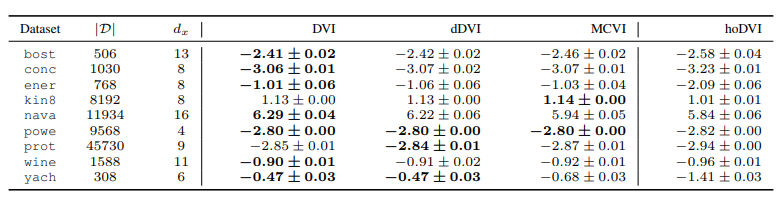
\includegraphics[scale=.45]{fig/results.png}
% \caption{Average log-likelihood on UCI datasets.}
% \end{figure}
\appendices
% \input{tex/Appendix.tex}



%==================================================================%
% References

% \bibliographystyle{cls/IEEEtran}
\bibliography{bib/ref}
\end{document}














